
%(BEGIN_QUESTION)
% Copyright 2006, Tony R. Kuphaldt, released under the Creative Commons Attribution License (v 1.0)
% This means you may do almost anything with this work of mine, so long as you give me proper credit

The Fisher model 846 I/P uses an interesting current-to-pressure transducer design, intended for use supplying variable-pressure air signals to position control valves.  A simplified diagram of its mechanism is shown here:

$$\includegraphics[width=15.5cm]{i00916x01.eps}$$

Explain how the feedback system works in this design, and how it differs substantially from classic pneumatic force-balance I/P transducer designs.

\underbar{file i00916}
%(END_QUESTION)





%(BEGIN_ANSWER)

The feedback loop in this I/P design is electronic, not mechanical.

%(END_ANSWER)





%(BEGIN_NOTES)

An inherent advantage of electronic feedback is that it is (potentially) more linear than mechanical feedback.  It is also noteworthy that the relay lies inside the feedback loop.  This means that negative feedback will automatically compensate for any inherent non-linearities within the relay.  Compare this with the Fisher model 546 I/P, where the pneumatic relay is not part of the feedback loop at all, and where the overall accuracy sensitively depends on relay performance.

%INDEX% Relay, I/P transducer: Fisher model 846

%(END_NOTES)


